\documentclass[aspectratio=169]{beamer}

% ---------- ENCODING & FONTS ----------
\usepackage[utf8]{inputenc}
\usepackage[T1]{fontenc}

% ---------- THEME & LOOK ----------
\usetheme{Madrid}
\usecolortheme{seahorse}
\usefonttheme{professionalfonts}
\setbeamertemplate{navigation symbols}{}
\setbeamercovered{transparent}
\setbeamertemplate{itemize items}[circle]
\setbeamertemplate{enumerate items}[default]
\setlength{\parskip}{0.25em}

% ---------- COLORS ----------
\usepackage{xcolor}
\definecolor{accent}{RGB}{0,92,184}
\definecolor{soft}{RGB}{233,244,255}
\definecolor{canadared}{RGB}{196,30,58}
\definecolor{leafgreen}{RGB}{0,130,80}
\definecolor{goldenrod}{RGB}{218,165,32}
\definecolor{deeporange}{RGB}{230,100,20}
\definecolor{ppfblue}{RGB}{30,100,200}
\definecolor{ppfred}{RGB}{200,50,50}
\definecolor{ppfgreen}{RGB}{30,160,80}
\setbeamercolor{structure}{fg=accent}
\setbeamercolor{title}{fg=white,bg=accent}
\setbeamercolor{frametitle}{fg=accent}
\setbeamercolor{block title}{bg=accent!12,fg=accent}
\setbeamercolor{block body}{bg=soft}

% ---------- PACKAGES ----------
\usepackage{booktabs}
\usepackage{amsmath, amssymb}
\usepackage{array}
\usepackage{hyperref}
\usepackage{tikz}
\usepackage{pgfplots}
\pgfplotsset{compat=1.18}
\usetikzlibrary{arrows.meta, positioning, decorations.pathreplacing, shapes.geometric, calc}
\hypersetup{colorlinks=true,linkcolor=accent,urlcolor=accent}

% ---------- SAFE TRANSITION FALLBACK ----------
\makeatletter
\@ifundefined{transfade}{\newcommand{\transfade}[1][]{}}{}
\makeatother

% ---------- TITLE ----------
\title{\textbf{Trade-offs, Comparative Advantage,\\ and the Market System}}
\subtitle{{\large ECON 101 -- Principles of Macroeconomics}}
\author{Muhebullah Karimzada}
\date{Spring 2026}

% ============================================================
\begin{document}
% ============================================================

\begin{frame}[plain]
  \titlepage
\end{frame}

% ============================================================
\begin{frame}{Chapter Outline}
\transfade
\begin{itemize}
  \item \textbf{2.1} Production Possibilities Frontiers and Opportunity Costs
  \item \textbf{2.2} Comparative Advantage and Trade
  \item \textbf{2.3} The Market System
\end{itemize}
\end{frame}

% ============================================================
\section{Scarcity and Trade-offs}
% ============================================================

\begin{frame}{Scarcity and Trade-offs}
\transfade
\begin{itemize}
  \item People continually face decisions about how best to use their \textbf{scarce} resources.
  \item \textbf{Scarcity:} a situation in which unlimited wants exceed the limited resources available to fulfill those wants.
  \item Scarcity requires \textbf{trade-offs}: to get more of one thing, society must accept less of another.
  \item Economics gives us tools to help make these trade-offs wisely.
\end{itemize}
\end{frame}

\begin{frame}{Canadian Example: Alberta's Energy Trade-off}
\transfade
\begin{itemize}
  \item Alberta has limited land, capital, and labour.
  \item If Alberta devotes more resources to \textbf{oil sands extraction}, fewer resources are available for \textbf{renewable energy} development (wind/solar).
  \item This trade-off is real: the Trans Mountain pipeline expansion (completed 2024) required massive capital that could have been invested elsewhere.
  \item \textbf{Source:} Natural Resources Canada; Statistics Canada Table 25-10-0063-01.
\end{itemize}
\end{frame}

% ============================================================
\section{2.1 Production Possibilities Frontiers and Opportunity Costs}
% ============================================================

\begin{frame}{2.1 Learning Objective}
\transfade
\begin{block}{Goal}
Use a production possibilities frontier to analyze opportunity costs and trade-offs.
\end{block}
\begin{itemize}
  \item A \textbf{production possibilities frontier (PPF)} is a curve showing the maximum attainable combinations of two goods that can be produced with available resources and current technology.
  \item The PPF is a \textbf{positive} tool: it shows what \emph{is} possible, not what \emph{should} be produced.
\end{itemize}
\end{frame}

%--- FIGURE 2.1 (1 of 2): Basic PPF ---
\begin{frame}{Figure 2.1 -- Canada's PPF: Oil vs.\ Clean Energy (1 of 2)}
\begin{center}
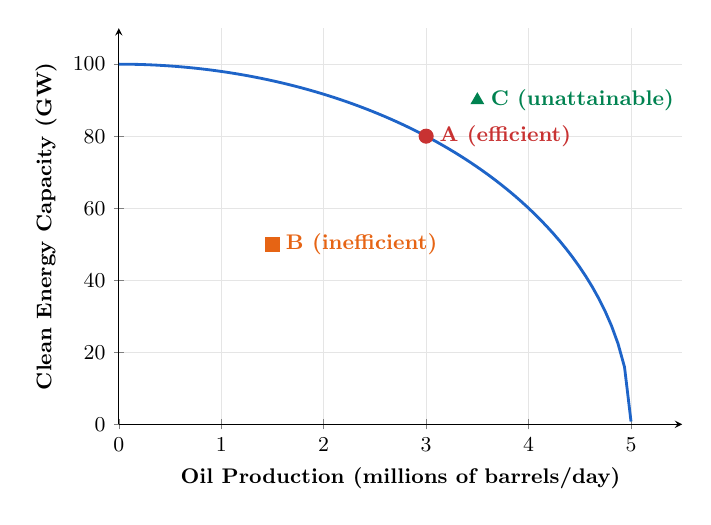
\begin{tikzpicture}[scale=0.85]
  \begin{axis}[
    width=10cm, height=7.5cm,
    xlabel={\textbf{Oil Production} (millions of barrels/day)},
    ylabel={\textbf{Clean Energy Capacity} (GW)},
    xmin=0, xmax=5.5,
    ymin=0, ymax=110,
    xtick={0,1,2,3,4,5},
    ytick={0,20,40,60,80,100},
    tick label style={font=\small},
    label style={font=\small\bfseries},
    axis lines=left,
    grid=major,
    grid style={gray!20},
    clip=false,
  ]
  % PPF curve: bowed out  y = 100*(1 - (x/5)^2)^0.5
  \addplot[very thick, color=ppfblue, domain=0:5, samples=80]
    {100*sqrt(1-(x/5)^2)};
  % Point A (efficient) -- (3,80) is exactly on the PPF: 100*sqrt(1-(3/5)^2)=80
  \addplot[mark=*, mark size=3pt, color=ppfred] coordinates {(3, 80)};
  \node[font=\small\bfseries, color=ppfred, right] at (axis cs:3.05,80) {A (efficient)};
  % Point B (inefficient) -- inside the PPF
  \addplot[mark=square*, mark size=3pt, color=deeporange] coordinates {(1.5,50)};
  \node[font=\small\bfseries, color=deeporange, right] at (axis cs:1.55,50) {B (inefficient)};
  % Point C (unattainable) -- outside the PPF (PPF at x=3.5 is ~71.4)
  \addplot[mark=triangle*, mark size=3pt, color=leafgreen] coordinates {(3.5,90)};
  \node[font=\small\bfseries, color=leafgreen, right] at (axis cs:3.55,90) {C (unattainable)};
  \end{axis}
\end{tikzpicture}
\end{center}
\end{frame}

\begin{frame}{Interpreting the PPF: Canada's Energy Sector}
\transfade
\begin{itemize}
  \item Canada's economy can produce combinations of \textbf{oil output} and \textbf{clean energy capacity}.
  \item \textbf{Point A} (on the PPF): productively efficient --- all resources are fully used.
  \item \textbf{Point B} (inside the PPF): attainable but \textbf{inefficient} --- idle workers or unused capital (e.g., pandemic-era shutdowns, 2020).
  \item \textbf{Point C} (outside the PPF): currently \textbf{unattainable} with existing resources and technology.
  \item \textbf{Data context:} Canada produced $\approx$4.9 million barrels/day of oil in 2024 and had $\approx$100 GW of total electricity capacity (Statistics Canada / NRCan).
\end{itemize}
\end{frame}

%--- FIGURE 2.1 (2 of 2): Opportunity cost movement ---
\begin{frame}{Figure 2.1 -- Moving Along the PPF: Opportunity Cost (2 of 2)}
\begin{center}
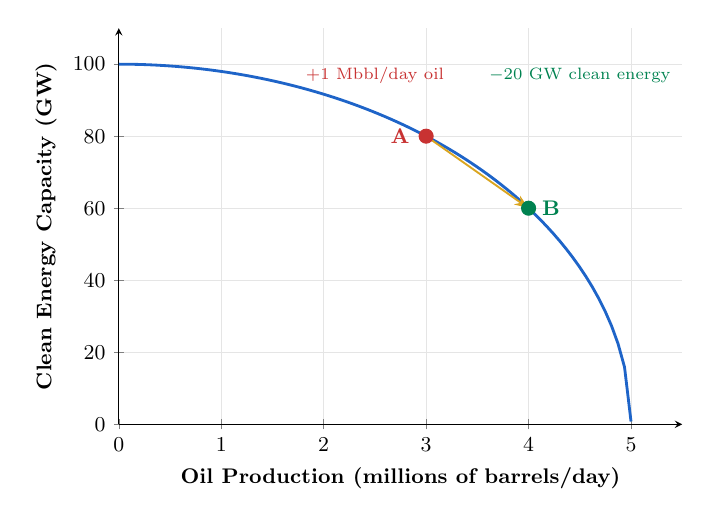
\begin{tikzpicture}[scale=0.85]
  \begin{axis}[
    width=10cm, height=7.5cm,
    xlabel={\textbf{Oil Production} (millions of barrels/day)},
    ylabel={\textbf{Clean Energy Capacity} (GW)},
    xmin=0, xmax=5.5,
    ymin=0, ymax=110,
    xtick={0,1,2,3,4,5},
    ytick={0,20,40,60,80,100},
    tick label style={font=\small},
    label style={font=\small\bfseries},
    axis lines=left,
    grid=major,
    grid style={gray!20},
    clip=false,
  ]
  \addplot[very thick, color=ppfblue, domain=0:5, samples=80]
    {100*sqrt(1-(x/5)^2)};
  % Point A at (3,80) -- exactly on the PPF
  \addplot[mark=*, mark size=3pt, color=ppfred] coordinates {(3,80)};
  \node[font=\small\bfseries, color=ppfred, left] at (axis cs:2.92,80) {A};
  % Point B at (4,60) -- exactly on the PPF: 100*sqrt(1-(4/5)^2)=60
  \addplot[mark=*, mark size=3pt, color=leafgreen] coordinates {(4,60)};
  \node[font=\small\bfseries, color=leafgreen, right] at (axis cs:4.05,60) {B};
  % Arrow
  \draw[-{Stealth[length=6pt]}, thick, color=goldenrod]
    (axis cs:3,80) -- (axis cs:4,60);
  % Annotation
  \node[font=\scriptsize, text=ppfred, align=center] at (axis cs:2.5,97)
    {+1 Mbbl/day oil};
  \node[font=\scriptsize, text=leafgreen, align=center] at (axis cs:4.5,97)
    {$-20$ GW clean energy};
  \end{axis}
\end{tikzpicture}
\end{center}
\vspace{-0.5em}
{\small Moving from A$\to$B: gaining 1 Mbbl/day of oil costs \textbf{20 GW of clean energy capacity} --- that is the opportunity cost.}
\end{frame}

\begin{frame}{Opportunity Cost on the PPF}
\transfade
\begin{itemize}
  \item Moving from point A to point B:
  \begin{itemize}
    \item Canada produces \textbf{1 million more barrels/day} of oil.
    \item To do so, it must give up \textbf{20 GW} of clean energy capacity.
  \end{itemize}
  \item The \textbf{opportunity cost} of that extra oil is the clean energy capacity sacrificed.
  \item \textbf{Opportunity cost:} the highest-valued alternative that must be given up to engage in an activity.
  \item Real-world context: the federal government's Clean Electricity Regulations (2024) explicitly recognize this trade-off.
\end{itemize}
\end{frame}

%--- FIGURE 2.2: Increasing marginal opportunity cost ---
\begin{frame}{Figure 2.2 -- Increasing Marginal Opportunity Costs}
\begin{center}
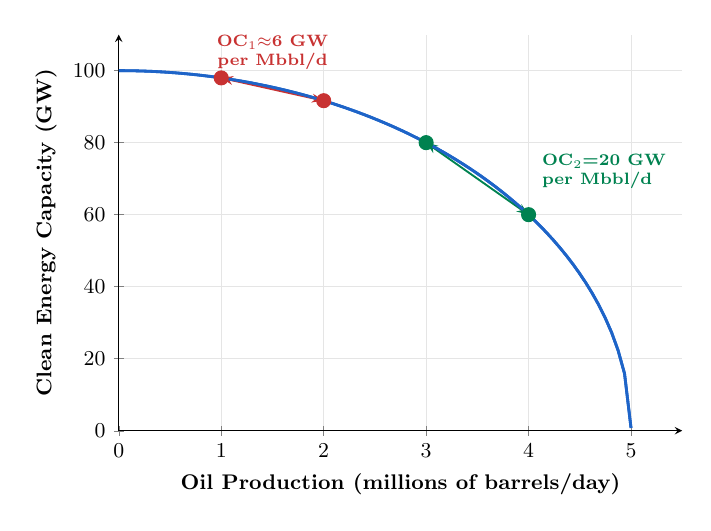
\begin{tikzpicture}[scale=0.85]
  \begin{axis}[
    width=10cm, height=7.5cm,
    xlabel={\textbf{Oil Production} (millions of barrels/day)},
    ylabel={\textbf{Clean Energy Capacity} (GW)},
    xmin=0, xmax=5.5,
    ymin=0, ymax=110,
    xtick={0,1,2,3,4,5},
    ytick={0,20,40,60,80,100},
    tick label style={font=\small},
    label style={font=\small\bfseries},
    axis lines=left,
    grid=major,
    grid style={gray!20},
    clip=false,
  ]
  \addplot[very thick, color=ppfblue, domain=0:5, samples=80]
    {100*sqrt(1-(x/5)^2)};
  % Segment 1: low OC -- (1,97.98) to (2,91.65) both on PPF
  % PPF at x=1: 100*sqrt(24/25)=97.98; at x=2: 100*sqrt(21/25)=91.65
  \addplot[mark=*, mark size=3pt, color=ppfred] coordinates {(1,97.98)};
  \addplot[mark=*, mark size=3pt, color=ppfred] coordinates {(2,91.65)};
  \draw[{Stealth[length=5pt]}-{Stealth[length=5pt]}, thick, color=ppfred]
    (axis cs:1,97.98) -- (axis cs:2,91.65);
  \node[font=\scriptsize\bfseries, color=ppfred, align=center] at (axis cs:1.5,105)
    {OC$_1$$\approx$6 GW\\per Mbbl/d};
  % Segment 2: higher OC -- (3,80) to (4,60) both on PPF (exact values)
  \addplot[mark=*, mark size=3pt, color=leafgreen] coordinates {(3,80)};
  \addplot[mark=*, mark size=3pt, color=leafgreen] coordinates {(4,60)};
  \draw[{Stealth[length=5pt]}-{Stealth[length=5pt]}, thick, color=leafgreen]
    (axis cs:3,80) -- (axis cs:4,60);
  \node[font=\scriptsize\bfseries, color=leafgreen, right, align=left] at (axis cs:4.05,72)
    {OC$_2$=20 GW\\per Mbbl/d};
  \addplot[very thick, color=ppfblue, domain=0:5, samples=80]
    {100*sqrt(1-(x/5)^2)};
  \end{axis}
\end{tikzpicture}
\end{center}
\end{frame}

\begin{frame}{Why Opportunity Costs Often Increase}
\transfade
\begin{itemize}
  \item Some resources are better suited to oil production, others to clean energy.
  \item The \emph{first} resources shifted from oil to clean energy are the ones \emph{most easily} repurposed.
  \item As more resources are diverted, the extra output gained falls --- giving the PPF its \textbf{bowed-out shape}.
  \item \textbf{Canadian example:} Shallow conventional oil fields in Saskatchewan are relatively easy to repurpose; deep oil sands operations in Alberta are highly specialized --- shifting them costs far more clean energy capacity.
\end{itemize}
\end{frame}

%--- FIGURE 2.3a: Economic Growth (outward shift) ---
\begin{frame}{Figure 2.3a -- Economic Growth: Outward Shift of the PPF}
\begin{center}
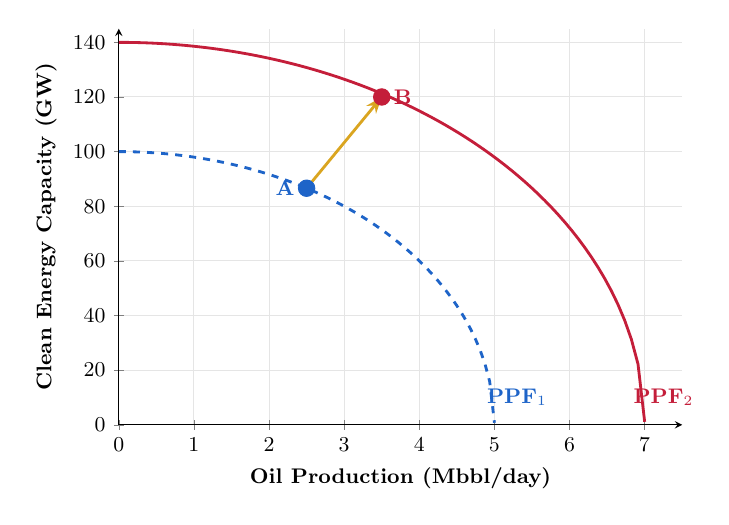
\begin{tikzpicture}[scale=0.85]
  \begin{axis}[
    width=10cm, height=7.5cm,
    xlabel={\textbf{Oil Production} (Mbbl/day)},
    ylabel={\textbf{Clean Energy Capacity} (GW)},
    xmin=0, xmax=7.5,
    ymin=0, ymax=145,
    xtick={0,1,2,3,4,5,6,7},
    ytick={0,20,40,60,80,100,120,140},
    tick label style={font=\small},
    label style={font=\small\bfseries},
    axis lines=left,
    grid=major,
    grid style={gray!20},
    clip=false,
  ]
  % Original PPF
  \addplot[very thick, color=ppfblue, domain=0:5, samples=80, dashed]
    {100*sqrt(1-(x/5)^2)};
  \node[font=\small\bfseries, color=ppfblue] at (axis cs:5.3,10) {PPF$_1$};
  % New PPF after growth
  \addplot[very thick, color=canadared, domain=0:7, samples=80]
    {140*sqrt(1-(x/7)^2)};
  \node[font=\small\bfseries, color=canadared] at (axis cs:7.25,10) {PPF$_2$};
  % Points A and B
  \addplot[mark=*, mark size=3.5pt, color=ppfblue] coordinates {(2.5,86.6)};
  \node[font=\small\bfseries, color=ppfblue, left] at (axis cs:2.45,86.6) {A};
  \addplot[mark=*, mark size=3.5pt, color=canadared] coordinates {(3.5,120)};
  \node[font=\small\bfseries, color=canadared, right] at (axis cs:3.55,120) {B};
  \draw[-{Stealth[length=7pt]}, very thick, color=goldenrod]
    (axis cs:2.5,86.6) -- (axis cs:3.5,120);
  \end{axis}
\end{tikzpicture}
\end{center}
\end{frame}

\begin{frame}{Economic Growth and the PPF}
\transfade
\begin{itemize}
  \item As more resources become available, the economy moves from A to B --- producing \textbf{more of both} goods.
  \item An \textbf{outward shift} of the PPF represents \textbf{economic growth}.
  \item \textbf{Economic growth:} the ability of the economy to increase the production of goods and services.
  \item \textbf{Canadian data:} Canada's real GDP grew by about 2.4\% per year on average 2000--2023 (Statistics Canada, CANSIM 36-10-0104-01). Each year, the PPF expanded outward.
  \item Macro link: long-run growth allows higher living standards without giving up other goods.
\end{itemize}
\end{frame}

%--- FIGURE 2.3b: Sector-specific technological change ---
\begin{frame}{Figure 2.3b -- Technological Change in One Sector}
\begin{center}
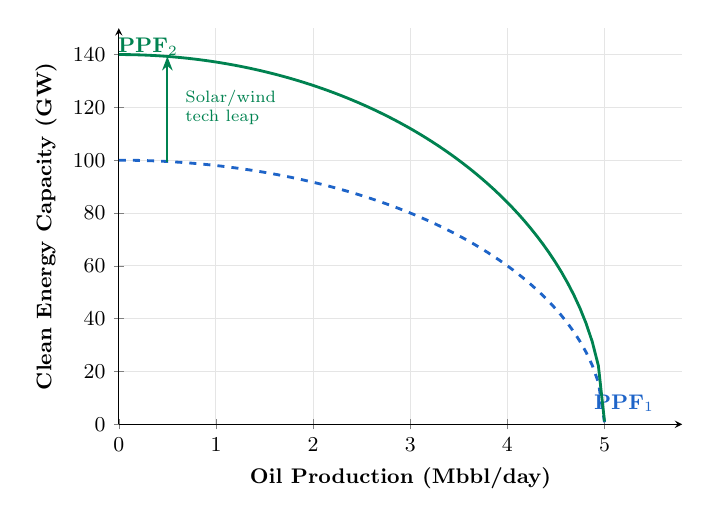
\begin{tikzpicture}[scale=0.85]
  \begin{axis}[
    width=10cm, height=7.5cm,
    xlabel={\textbf{Oil Production} (Mbbl/day)},
    ylabel={\textbf{Clean Energy Capacity} (GW)},
    xmin=0, xmax=5.8,
    ymin=0, ymax=150,
    xtick={0,1,2,3,4,5},
    ytick={0,20,40,60,80,100,120,140},
    tick label style={font=\small},
    label style={font=\small\bfseries},
    axis lines=left,
    grid=major,
    grid style={gray!20},
    clip=false,
  ]
  % PPF1 (original, dashed)
  \addplot[very thick, color=ppfblue, domain=0:5, samples=80, dashed]
    {100*sqrt(1-(x/5)^2)};
  \node[font=\small\bfseries, color=ppfblue] at (axis cs:5.2,8) {PPF$_1$};
  % PPF2: clean energy tech improves -- y-intercept expands to 140, x-intercept same
  \addplot[very thick, color=leafgreen, domain=0:5, samples=80]
    {140*sqrt(1-(x/5)^2)};
  \node[font=\small\bfseries, color=leafgreen] at (axis cs:0.3,143) {PPF$_2$};
  % Arrow showing vertical expansion at x=0.5
  \draw[-{Stealth[length=6pt]}, thick, color=leafgreen]
    (axis cs:0.5,99.5) -- (axis cs:0.5,139.3);
  \node[font=\scriptsize, color=leafgreen, right, align=left] at (axis cs:0.6,120)
    {Solar/wind\\tech leap};
  \end{axis}
\end{tikzpicture}
\end{center}
\end{frame}

\begin{frame}{Technological Change in One Industry}
\transfade
\begin{itemize}
  \item Suppose technology improves in \textbf{clean energy only} (e.g., cheaper solar panels, better battery storage).
  \item The maximum clean energy capacity increases, but the oil production frontier is unchanged.
  \item Previously unattainable combinations become attainable.
  \item \textbf{Canadian example:} The cost of utility-scale solar in Canada dropped by $\approx$89\% from 2010 to 2023, allowing the clean energy PPF frontier to expand significantly (IRENA / NRCan data).
\end{itemize}
\end{frame}

% ============================================================
\section{2.2 Comparative Advantage and Trade}
% ============================================================

\begin{frame}{2.2 Learning Objective}
\transfade
\begin{block}{Goal}
Understand comparative advantage and explain how it serves as the basis for trade.
\end{block}
\end{frame}

\begin{frame}{Canada--USA Trade Example}
\transfade
\begin{itemize}
  \item Canada and the USA each have limited land, labour, and capital.
  \item Suppose both can produce \textbf{wheat} and \textbf{aircraft}.
  \item \textbf{In one year}, with all resources devoted to one good:
  \begin{itemize}
    \item \textbf{Canada:} 300 Mt of wheat \emph{or} 150 aircraft.
    \item \textbf{USA:} 900 Mt of wheat \emph{or} 600 aircraft.
  \end{itemize}
  \item The USA is \textbf{absolutely} better at producing both.
  \item Yet both countries can \textbf{still gain} from trade --- the key is \textbf{comparative advantage}.
\end{itemize}
\end{frame}

%--- FIGURE 2.4: PPFs without trade ---
\begin{frame}{Figure 2.4 -- Canada \& USA PPFs Without Trade}
\begin{columns}
\column{0.5\textwidth}
\begin{center}
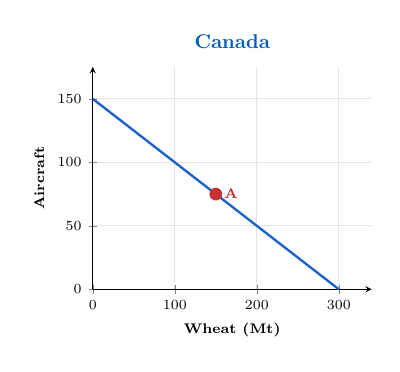
\begin{tikzpicture}[scale=0.72]
  \begin{axis}[
    width=6.5cm, height=5.5cm,
    title={\textbf{\color{accent}Canada}},
    xlabel={Wheat (Mt)},
    ylabel={Aircraft},
    xmin=0, xmax=340,
    ymin=0, ymax=175,
    xtick={0,100,200,300},
    ytick={0,50,100,150},
    tick label style={font=\scriptsize},
    label style={font=\scriptsize\bfseries},
    axis lines=left,
    grid=major, grid style={gray!20},
    clip=false,
  ]
  \addplot[very thick, color=ppfblue] coordinates {(0,150)(300,0)};
  % Autarky point A: wheat=150, aircraft=75
  \addplot[mark=*, mark size=3pt, color=ppfred] coordinates {(150,75)};
  \node[font=\scriptsize\bfseries, color=ppfred, right] at (axis cs:152,75) {A};
  \end{axis}
\end{tikzpicture}
\end{center}

\column{0.5\textwidth}
\begin{center}
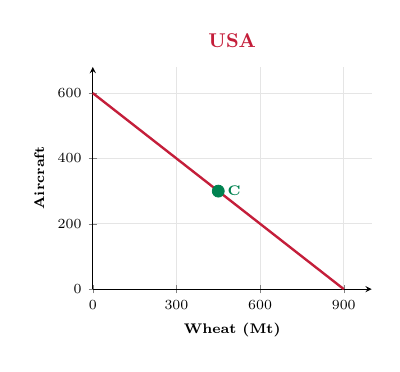
\begin{tikzpicture}[scale=0.72]
  \begin{axis}[
    width=6.5cm, height=5.5cm,
    title={\textbf{\color{canadared}USA}},
    xlabel={Wheat (Mt)},
    ylabel={Aircraft},
    xmin=0, xmax=1000,
    ymin=0, ymax=680,
    xtick={0,300,600,900},
    ytick={0,200,400,600},
    tick label style={font=\scriptsize},
    label style={font=\scriptsize\bfseries},
    axis lines=left,
    grid=major, grid style={gray!20},
    clip=false,
  ]
  \addplot[very thick, color=canadared] coordinates {(0,600)(900,0)};
  % Autarky point C: wheat=450, aircraft=300
  \addplot[mark=*, mark size=3pt, color=leafgreen] coordinates {(450,300)};
  \node[font=\scriptsize\bfseries, color=leafgreen, right] at (axis cs:458,300) {C};
  \end{axis}
\end{tikzpicture}
\end{center}
\end{columns}
\vspace{0.4em}
\centering\small Without trade, each country consumes only what it produces (points A and C).
\end{frame}

\begin{frame}{Autarky (No Trade) Outcomes}
\transfade
\begin{itemize}
  \item Without trade, each country consumes only what it produces.
  \item \textbf{Canada (Point A):} produces and consumes 150 Mt wheat and 75 aircraft.
  \item \textbf{USA (Point C):} produces and consumes 450 Mt wheat and 300 aircraft.
  \item Both are on their own PPFs, but \emph{neither} is at the best possible consumption point once trade is allowed.
\end{itemize}
\end{frame}

\begin{frame}{Specialization and Gains from Trade}
\transfade
\begin{itemize}
  \item \textbf{Trade:} the act of buying and selling across borders.
  \item The USA is absolutely better at producing both wheat and aircraft.
  \item But each country should specialize in what it is \textbf{relatively} better at.
  \item The key concept: \textbf{comparative advantage} --- produce where your \emph{opportunity cost} is lower.
\end{itemize}
\end{frame}

%--- TABLE 2.1 (built in LaTeX) ---
\begin{frame}{Table 2.1 -- Opportunity Costs of Wheat and Aircraft}
\begin{center}
\renewcommand{\arraystretch}{1.6}
\begin{tabular}{lcc}
\toprule
 & \textbf{\color{accent}Canada} & \textbf{\color{canadared}USA} \\
\midrule
\textbf{OC of 1 Mt wheat} & $\tfrac{150}{300}=0.5$ aircraft & $\tfrac{600}{900}=0.67$ aircraft \\
\textbf{OC of 1 aircraft} & $\tfrac{300}{150}=2$ Mt wheat & $\tfrac{900}{600}=1.5$ Mt wheat \\
\midrule
\textbf{Comparative advantage in:} & \textcolor{ppfblue}{\textbf{Wheat}} & \textcolor{canadared}{\textbf{Aircraft}} \\
\bottomrule
\end{tabular}
\end{center}
\vspace{0.5em}
\begin{block}{Key insight}
Canada gives up \emph{less} to produce wheat; the USA gives up \emph{less} to produce aircraft.
\end{block}
\end{frame}

%--- FIGURE 2.5: Gains from trade ---
\begin{frame}{Figure 2.5 -- Gains from Trade}
\begin{columns}
\column{0.5\textwidth}
\begin{center}
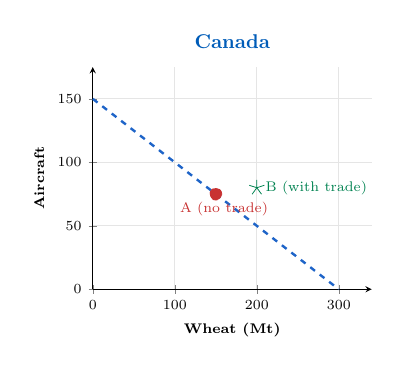
\begin{tikzpicture}[scale=0.72]
  \begin{axis}[
    width=6.5cm, height=5.5cm,
    title={\textbf{\color{accent}Canada}},
    xlabel={Wheat (Mt)},
    ylabel={Aircraft},
    xmin=0, xmax=340,
    ymin=0, ymax=175,
    xtick={0,100,200,300},
    ytick={0,50,100,150},
    tick label style={font=\scriptsize},
    label style={font=\scriptsize\bfseries},
    axis lines=left,
    grid=major, grid style={gray!20},
    clip=false,
  ]
  \addplot[very thick, color=ppfblue, dashed] coordinates {(0,150)(300,0)};
  % Specialization: Canada produces (300,0), trades 100Mt wheat for 80 aircraft
  % Consumption B: (200, 80) -- outside old PPF
  \addplot[mark=*, mark size=3pt, color=ppfred, dashed] coordinates {(150,75)};
  \node[font=\scriptsize, color=ppfred] at (axis cs:160,63) {A (no trade)};
  \addplot[mark=star, mark size=4pt, color=leafgreen] coordinates {(200,80)};
  \node[font=\scriptsize, color=leafgreen, right] at (axis cs:202,80) {B (with trade)};
  \end{axis}
\end{tikzpicture}
\end{center}

\column{0.5\textwidth}
\begin{center}
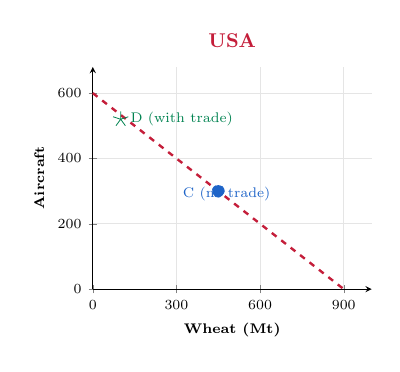
\begin{tikzpicture}[scale=0.72]
  \begin{axis}[
    width=6.5cm, height=5.5cm,
    title={\textbf{\color{canadared}USA}},
    xlabel={Wheat (Mt)},
    ylabel={Aircraft},
    xmin=0, xmax=1000,
    ymin=0, ymax=680,
    xtick={0,300,600,900},
    ytick={0,200,400,600},
    tick label style={font=\scriptsize},
    label style={font=\scriptsize\bfseries},
    axis lines=left,
    grid=major, grid style={gray!20},
    clip=false,
  ]
  \addplot[very thick, color=canadared, dashed] coordinates {(0,600)(900,0)};
  \addplot[mark=*, mark size=3pt, color=ppfblue, dashed] coordinates {(450,300)};
  \node[font=\scriptsize, color=ppfblue] at (axis cs:480,290) {C (no trade)};
  % USA specializes in aircraft (600), receives 100Mt wheat
  % Consumption D: (100+100, 600-80) = actually (100, 520)
  \addplot[mark=star, mark size=4pt, color=leafgreen] coordinates {(100,520)};
  \node[font=\scriptsize, color=leafgreen, right] at (axis cs:110,520) {D (with trade)};
  \end{axis}
\end{tikzpicture}
\end{center}
\end{columns}
\vspace{0.3em}
\centering\small Both countries reach consumption points \textbf{outside} their own PPFs --- gains from trade!
\end{frame}

%--- TABLE 2.2: Gains summary ---
\begin{frame}{Table 2.2 -- Summary of the Gains from Trade}
\begin{center}
\renewcommand{\arraystretch}{1.5}
\begin{tabular}{lcccc}
\toprule
 & \multicolumn{2}{c}{\textbf{\color{accent}Canada}} & \multicolumn{2}{c}{\textbf{\color{canadared}USA}} \\
\cmidrule(lr){2-3}\cmidrule(lr){4-5}
 & Wheat (Mt) & Aircraft & Wheat (Mt) & Aircraft \\
\midrule
\textbf{Without trade} & 150 & 75 & 450 & 300 \\
\textbf{With trade} & \textcolor{ppfgreen}{\textbf{200}} & \textcolor{ppfgreen}{\textbf{80}} & \textcolor{ppfgreen}{\textbf{100}} & \textcolor{ppfgreen}{\textbf{520}} \\
\textbf{Gain} & \textcolor{leafgreen}{+50} & \textcolor{leafgreen}{+5} & \textcolor{leafgreen}{--} & \textcolor{leafgreen}{+220} \\
\bottomrule
\end{tabular}
\end{center}
\vspace{0.5em}
\begin{block}{Key lesson}
Both countries consume \emph{more} with trade --- even though the USA is absolutely better at producing everything.
\end{block}
\end{frame}

\begin{frame}{Explaining the Gains from Trade}
\transfade
\begin{itemize}
  \item The USA has an \textbf{absolute advantage} in both wheat and aircraft.
  \item Canada has a \textbf{comparative advantage} in wheat (lower opportunity cost).
  \item The USA has a \textbf{comparative advantage} in aircraft.
  \item \textbf{Absolute advantage:} the ability to produce more of a good using the same resources.
  \item \textbf{Comparative advantage:} the ability to produce a good at a \emph{lower opportunity cost}.
  \item Real context: Canada exports $\approx$\$12B of wheat/canola annually; the USA exports $\approx$\$130B of aerospace products (Statistics Canada; U.S. BEA, 2023).
\end{itemize}
\end{frame}

\begin{frame}{Canada's Comparative Advantages Today}
\transfade
\begin{itemize}
  \item \textbf{Natural resources:} potash, lumber, oil, canola, uranium --- Canada is a low-opportunity-cost producer.
  \item \textbf{Financial services:} Canadian banks are globally competitive.
  \item \textbf{AI \& technology:} the ``Toronto--Waterloo corridor'' and Montreal AI cluster reflect a comparative advantage in AI research.
  \item \textbf{High opportunity cost goods:} electronics assembly, consumer goods --- Canada imports these from countries with comparative advantages there.
  \item \textbf{Source:} Statistics Canada, International Trade Division; Bank of Canada Business Outlook Survey, 2024.
\end{itemize}
\end{frame}

% ============================================================
\section{2.3 The Market System}
% ============================================================

\begin{frame}{2.3 Learning Objective}
\transfade
\begin{block}{Goal}
Explain the basic idea of how a market system works.
\end{block}
\end{frame}

\begin{frame}{Markets and the Modern Economy}
\transfade
\begin{itemize}
  \item A \textbf{market} is a group of buyers and sellers of a good or service, and the institution or arrangement by which they come together to trade.
  \item Two key groups participate in the modern economy:
  \begin{itemize}
    \item \textbf{Households}
    \item \textbf{Firms}
  \end{itemize}
  \item \textbf{Canadian context:} Canada has $\approx$15 million households and $\approx$1.2 million employer businesses (Statistics Canada, 2024).
\end{itemize}
\end{frame}

\begin{frame}{Households and Firms}
\transfade
\begin{itemize}
  \item \textbf{Households} consist of individuals who provide \textbf{factors of production}:
  \begin{itemize}
    \item labour, capital, natural resources, and entrepreneurial ability.
  \end{itemize}
  \item Households receive payments for these factors by selling them to firms in \textbf{factor markets}.
  \item \textbf{Firms} supply goods and services to \textbf{product markets}; households buy these from firms.
\end{itemize}
\end{frame}

\begin{frame}{The Four Factors of Production}
\transfade
\begin{itemize}
  \item \textbf{Labour:} all types of work --- from baristas at Tim Hortons to executives at RBC.
  \item \textbf{Capital:} machines, buildings, computers --- e.g., pipelines, data centres, manufacturing plants.
  \item \textbf{Natural resources:} land, water, oil sands, forests, mineral deposits.
  \item \textbf{Entrepreneurial ability:} organizing the other factors to create value --- e.g., founding a startup on the Toronto--Waterloo corridor.
  \item \textbf{Source:} Statistics Canada, Labour Force Survey; Bank of Canada, Monetary Policy Report (April 2025).
\end{itemize}
\end{frame}

%--- FIGURE 2.6: Circular-flow diagram (TikZ) ---
\begin{frame}{Figure 2.6 -- The Circular-Flow Diagram}
\begin{center}
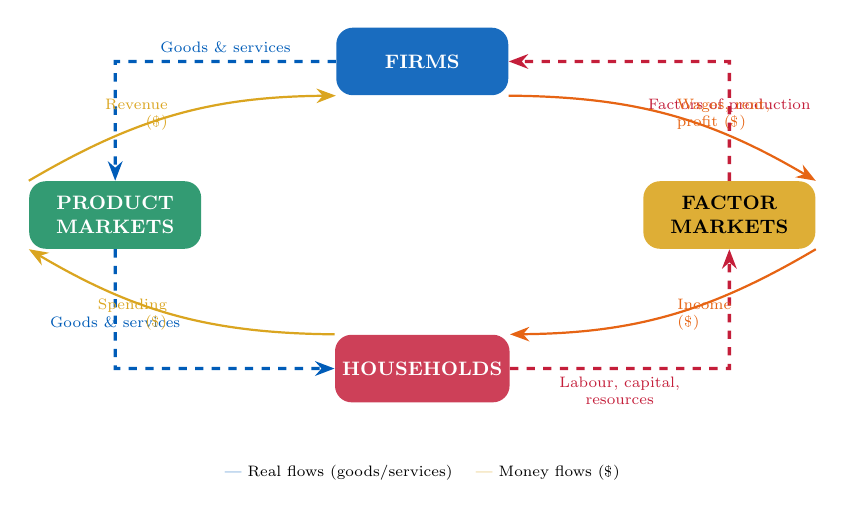
\begin{tikzpicture}[
  box/.style={rectangle, rounded corners=6pt, minimum width=2.8cm,
              minimum height=1.1cm, align=center, font=\small\bfseries},
  scale=0.78, transform shape
]
  % Boxes
  \node[box, fill=accent!90, text=white] (firms)      at (0, 2.5)  {FIRMS};
  \node[box, fill=canadared!85, text=white] (hh)       at (0,-2.5)  {HOUSEHOLDS};
  \node[box, fill=leafgreen!80, text=white] (product)  at (-5, 0)  {PRODUCT\\MARKETS};
  \node[box, fill=goldenrod!90, text=black]  (factor)   at ( 5, 0)  {FACTOR\\MARKETS};

  % Real flows (outer, dashed)
  % Goods/services: Firms -> Product Markets -> Households
  \draw[-{Stealth[length=7pt]}, very thick, color=accent, dashed]
    (firms.west) -- (-5,2.5) node[midway, above, font=\scriptsize, text=accent]{Goods \& services} -- (product.north);
  \draw[-{Stealth[length=7pt]}, very thick, color=accent, dashed]
    (product.south) -- (-5,-2.5) node[midway, below, font=\scriptsize, text=accent]{Goods \& services} -- (hh.west);

  % Factors: Households -> Factor Markets -> Firms
  \draw[-{Stealth[length=7pt]}, very thick, color=canadared, dashed]
    (hh.east) -- (5,-2.5) node[midway, below, font=\scriptsize, text=canadared, align=center]{Labour, capital,\\resources} -- (factor.south);
  \draw[-{Stealth[length=7pt]}, very thick, color=canadared, dashed]
    (factor.north) -- (5,2.5) node[midway, above, font=\scriptsize, text=canadared, align=center]{Factors of production} -- (firms.east);

  % Money flows (inner, solid)
  \draw[-{Stealth[length=7pt]}, thick, color=goldenrod]
    (hh.north west) to[bend left=15] node[midway, left, font=\scriptsize, text=goldenrod, align=right]{Spending\\(\$)} (product.south west);
  \draw[-{Stealth[length=7pt]}, thick, color=goldenrod]
    (product.north west) to[bend left=15] node[midway, left, font=\scriptsize, text=goldenrod, align=right]{Revenue\\(\$)} (firms.south west);
  \draw[-{Stealth[length=7pt]}, thick, color=deeporange]
    (firms.south east) to[bend left=15] node[midway, right, font=\scriptsize, text=deeporange, align=left]{Wages, rent,\\profit (\$)} (factor.north east);
  \draw[-{Stealth[length=7pt]}, thick, color=deeporange]
    (factor.south east) to[bend left=15] node[midway, right, font=\scriptsize, text=deeporange, align=left]{Income\\(\$)} (hh.north east);

  % Legend
  \node[font=\scriptsize, align=left] at (0,-4.2)
    {\textcolor{accent}{---} Real flows (goods/services) \quad
     \textcolor{goldenrod}{---} Money flows (\$)};
\end{tikzpicture}
\end{center}
\end{frame}

\begin{frame}{Circular-Flow Diagram: Basic Idea}
\transfade
\begin{itemize}
  \item The \textbf{circular-flow diagram} illustrates how participants in markets are linked.
  \item \textbf{Real flows:}
  \begin{itemize}
    \item Households provide factors of production to firms.
    \item Firms provide goods and services to households.
  \end{itemize}
  \item \textbf{Money flows:}
  \begin{itemize}
    \item Firms pay wages, rent, and profits to households for factors.
    \item Households pay for goods and services from firms.
  \end{itemize}
  \item \textbf{Canadian scale:} Total household spending $\approx$\$1.7 trillion in 2024 (Statistics Canada, National Accounts).
\end{itemize}
\end{frame}

\begin{frame}{Limits of the Simple Circular-Flow Model}
\transfade
\begin{itemize}
  \item Like all economic models, the circular-flow diagram is a \textbf{simplified} version of reality.
  \item The basic version excludes:
  \begin{itemize}
    \item \textbf{Government} (taxes, transfers, public services)
    \item \textbf{Financial system} (Bank of Canada, chartered banks, credit markets)
    \item \textbf{Foreign sector} (exports, imports, exchange rates)
  \end{itemize}
  \item We add all three sectors in later chapters to build full macroeconomic models.
\end{itemize}
\end{frame}

\begin{frame}{Gains from Free Markets}
\transfade
\begin{itemize}
  \item A \textbf{free market} has few government restrictions on how goods or services can be produced, sold, or how factors can be employed.
  \item Countries closer to this benchmark have generally raised living standards faster.
  \item Adam Smith's \textbf{``invisible hand''}: individuals pursuing self-interest collectively coordinate economic activity.
  \item \textbf{Canadian context:} Canada ranks among the top 10 in the World Bank's Ease of Doing Business index; free trade agreements (CUSMA, CPTPP) have expanded market access for Canadian producers.
\end{itemize}
\end{frame}

% ============================================================
\section{Things to Remember \& Summary}
% ============================================================

\begin{frame}{Things to Remember}
\transfade
\begin{itemize}
  \item The PPF should \textbf{never bow inward} --- opportunity cost is non-decreasing.
  \item The PPF tells us what \textbf{can} be produced, not what \textbf{should} be produced.
  \item Someone being better at \emph{everything} does \textbf{not} eliminate gains from trade.
  \item The basis for trade is \textbf{comparative advantage}, not absolute advantage.
  \item Free markets raise living standards, but governments must provide a sound legal environment (property rights, contract enforcement) for markets to function.
\end{itemize}
\end{frame}

\begin{frame}{Chapter Summary}
\transfade
\begin{itemize}
  \item PPFs illustrate trade-offs, opportunity cost, economic growth, and technological change.
  \item \textbf{Comparative advantage} explains why Canada, the USA, and other nations gain from specialization and trade.
  \item The \textbf{market system} coordinates decisions of millions of households and firms through product and factor markets.
  \item The \textbf{circular-flow diagram} provides a macro picture of how goods, services, and money move in the economy.
  \item Free markets and well-functioning institutions are central to long-run improvements in living standards.
\end{itemize}
\end{frame}

\begin{frame}
\centering
\Huge \textbf{Thank you!}\\[1em]
\normalsize Questions? \\[0.5em]
\small \textit{Data sources: Statistics Canada, Bank of Canada, Natural Resources Canada, NRCan, IRENA}
\end{frame}

\end{document}
